
\section{Serverová část}
Tato sekce popisuje návrh a realizaci serverového řešení včetně architektury, implementovaných bezpečnostních mechanizmů a definici schématu pro komunikaci s platformou na protokolu MQTT.


\subsection{Architektura}
Systém implementuje relaxovanou \textbf{Třívrstvou architekturu} obohacenou o vzor \textbf{Publish subscribe}. Základní myšlenkou Třívrstvé architektury je oddělení zodpovědnosti do tří vrstev, kde každá vrstva by měla být zodpovědná za určitou činnost a nepřesahovat svým rozsahem do zodpovědnosti jiné. Jednotlivé vrstvy:
\begin{itemize}
    \item Controller (řadič) - prostředník pro komunikaci mezi uživatelským rozhraním a služeb, které systém nabízí.
    \item Service (služba) - část systému obsahující aplikační logiku, jejímž úkolem je vykonání určitých úkolů (např. vytvoření uživatele).
    \item Data access layer (vrstva pro přístup k datům) - vrstva zapouzdřující přístup do databáze, která vytváří dle požadavků příslušné dotazy a výsledky mapuje na objekty, se kterými se pracuje lépe než s textovými záznamy.
\end{itemize}

Vzor \textbf{Publish subscribe} přidává navíc asynchronní zpracování událostí. Toto řešení je velmi užitečné v případě, pokud je potřeba navázat nějaké akce (nejčastěji volání třetí strany např. kvůli analytickým údajům). Například pokud vytvoříme řadič pro registraci uživatele, tak od něj očekáváme, že vytvoří uživatele a to je vše. Jsou ale situace kdy potřebujeme navázat další akce, které nemají žádnou přímou spojitost s danou odpovědností (např. zalogování do google Analytics nebo odeslání emailu). Přidáním této akce přímo do kontrolleru bychom porušili \textit{Princip jedné odpovědnosti} (Single-responsibility principle), který říká, že každý objekt (v tomto případě řadič) by měl vykonávat pouze činnost, která se od něj očekává. V tuto chvíli se hodí vzor \textit{Publish subscribe}, který umožní v řadiči vyslání (emit) události, že byl registrován uživatel a veškeré nesouvisející akce se vykonají v obsluze dané události v jiné části systému. Díky tomu nedojde k porušení Principu jedné odpovědnosti a kód řadiče dělá přesně to, co se od něj očekává a nic víc.

Serverová část je rozdělena na dva separátní procesy kvůli zvýšení odolnosti, aby v případě pádu jedné z části buď fungovalo uživatelské rozhraní nebo část obsluhující komunikaci se zařízeními.
\begin{itemize}
    \item \textbf{Backend} - dává k dispozici RESTful rozhraní pro kompletní ovládání platformy, dále vykonává naplánová akce jako odesílání emailů.
    \item \textbf{Backend-mqtt} - interaguje se zařízeními přes MQTT broker a odesílá real-time změny na frontend.
\end{itemize}

\begin{figure}[htbp]
    \label{packages-uml}
    \centering
    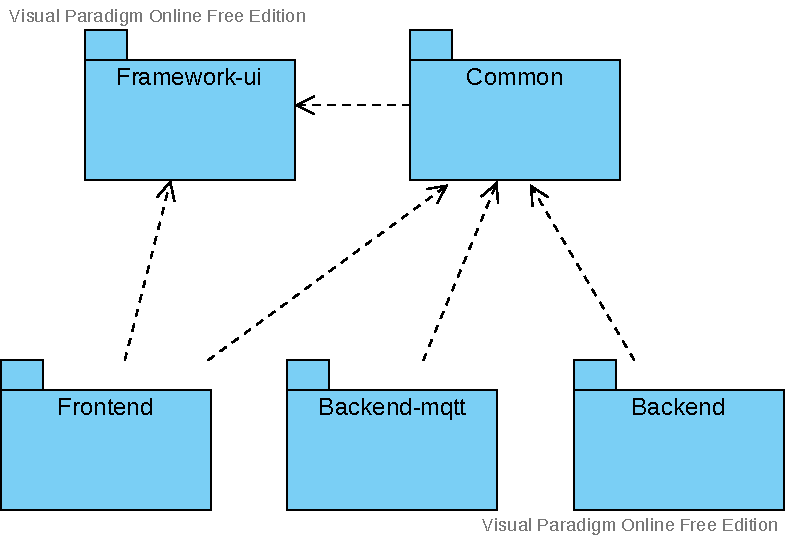
\includegraphics[width=0.5\textwidth]{img/packages.pdf}
    \caption{Diagram rozdělení balíčků}
\end{figure}

\subsection{Databáze}
Databáze je kritická část každého systému, protože se stará o perzistentní uchování dat, bez kterého bychom ztratili veškerá data při restartu či výpadku elektrické energie. Databáze lze obecně rozdělit do dvou skupin. První je označována jako SQL, která je založená na předpokladu, že objekty (reálného či virtuálního světa) lze přesně definovat a zpravidla mají mezi sebou vztah (relaci) např. potraviny a nákupní košík - vložení potravin do košíku lze reprezentovat vztahem, který je mezi danou potravinou a košíkem (je vložena / není). SQL databáze se orientují právě na zachycení vztahů mezi strukturovanými daty. Naopak druhá skupina NoSQL (Not only SQL) se orientuje na ukládání nerelačních nestrukturovaných dat. Problematika různých typů databází je velice rozsáhlá a více se jí zde věnovat nebudeme. Pro podrobnější popis doporučuji \cite{sql-and-nosql}.

Oba přístupy mají své výhody a nevýhody. Je potřeba vždy volit databázi na základě druhu dat, která budou uchovávat. Pro mé řešení jsem zvolil NoSQL databázi z následujících důvodů. Vzájemná provázanost dat bude naprosto minimální viz. sekce s doménovým modelem \ref{domain-model}. Dále zařízení mohou produkovat potencionálně obrovské množství dat, pro což se NoSQL databáze hodí lépe, protože umožnují tzv. horizontální škálování (rozložení zátěže na více fyzických strojů), které pro SQL databáze lze efektivně využít pouze pro čtení nikoliv zápis. NoSQL databáze také umožňuje mnohem dynamičtější vývoj, protože SQL databáze vyžadují pevnou strukturu dat a i malá změna struktury znamená často velmi složitou migraci všech dat, zatímco NoSQL databáze umožňují ukládání dat bez nutnosti definovat jejich strukturu.

Specificky byla zvolena NoSQL databáze MongoDB, která je velmi populární mezi vývojáři, má skvělou podporu ze strany knihoven v NodeJS světě a pro uchovávání dat používá formát podobný formátu JSON (MongoDB nazývá formát BSON \cite{bson-vs-json}), což se velmi snadno kombinuje s jazykem JavaScript, který JSON používá pro nativní objekty.

\paragraph{Mongoose} je knihovna pro NodeJS, která vytváří nad MongoDB objektovou abstrakci a spoustu dalších užitečných funkcí jako validace a type cast \cite{mongoose}. Základním prvkem je definování schéma pro jednotlivé dokumenty, což může vypadat jako návrat do striktního schématu u SQL databází, ale zde je schéma definované pouze na úrovni Mongoose, tedy mnohem flexibilnější a méně restriktivní. MongoDB nabízí oficiální knihovnu pro přístup do databáze, ale preferuji Mongoose, protože díky definici schémat mám obecně větší kontrolu nad daty, která se dostanou do databáze a mají výbornou rozsáhlou dokumentaci.

\subsection{Souborová struktura}
Oba procesy jsou rozděleny do separátních balíčků \textit{backend} a \textit{backend-mqtt}, které na sobě nejsou nijak závislé a pro sdílení společných částí kódu, primárně databázových modelů, je využíván balíček \textbf{common}. Následující souborová struktura pro oba procesy byla inspirována článkem \textit{Bulletproof node.js project architecture} \cite{bolletproof-architecture}, která se mi velmi osvědčila v jiných projektech.
\dirtree{%
    .1 packages.
    .2 backend\DTcomment{obsluha RESTful rozhraní a úkolů}.
    .3 src.
    .4 api\DTcomment{zdrojové kódy pro jednotlivé endpointy}.
    .5 device.
    .5 discovery.
    .5 user.
    .4 jobs\DTcomment{definice úkolů pro AgendaJS}.
    .4 loaders\DTcomment{rozdělený startovací proces do modulů}.
    .4 middleware\DTcomment{definice vlastních middleware}.
    .4 services\DTcomment{zdrojové kódy služeb}.
    .4 subscribers\DTcomment{obsluha akcí na asynchroní události}.
    .2 backend-mqtt\DTcomment{oblsuha MQTT a Socket.IO}.
    .3 src.
    .4 api.
    .5 auth\DTcomment{endpoint pro RabbitMQ autentifikaci}.
    .5 actions\DTcomment{endpoint pro interní komunikaci s Backend}.
    .4 services\DTcomment{zdrojové kódy služeb}.
    .5 firebase\DTcomment{odesílání notifikací}.
    .5 mqtt\DTcomment{napojení na MQTT broker a obsluhu zařízení}.
    .5 websocket\DTcomment{real-time komunikace pomocí Socket.IO}.
    .4 subscribers\DTcomment{definice akcí na asynchroní události}.
    .2 common\DTcomment{obsahuje sdílené části kódu}.
    .3 src.
    .4 config\DTcomment{konfigurace načtená z promněných prostředí}.
    .4 models\DTcomment{definice mongoose schémat a typů}.
    .4 utils.
}


\subsection{Proces Backend}
Tento proces s využitím frameworku \hyperref[expressjs]{ExpressJS} implementuje webový server nabízející RESTful rozhraní pro vytváření, editaci a mazání všech entit platformy. Data se odesílají a konzumují ve formátu JSON. Proces dále implementuje odesílání emailů.

\subsubsection{Popis rozhraní}
Všechny endpointy, až na přihlášení a registraci uživatele, vyžadují autentizační token v hlavičce požadavku. Odpověď se potom liší podle oprávnění daného uživatele. Ukázka rozhraní:
\begin{itemize}
    \item POST /user - vytvoří nového uživatele
    \item GET /device - vrací seznam zařízení
    \item DELETE /device/:deviceId - odstraní dané zařízení
    \item PATCH /device/:deviceId - aktualizuje zařízení
    \item GET /device/:deviceId/thing/:thingId/history?from=\&to - vrací historická data pro specifikovanou věc, parametry specifikují časový rozsah
    \item PUT /device/:deviceId/thing/:thingId/notify - nastaví notifikační pravidla pro určitou věc
    \item PATCH /device/:deviceId/thing/:thingId - aktualizuje state pro danou věc
\end{itemize}

Server na požadavky odpovídá následujícími HTTP kódy (tělo odpovědi obsahuje podrobnější chybovou hlášku):
\begin{itemize}
    \item 200 - v pořádku, součástí těla odpovědi jsou data
    \item 204 - v pořádku, tělo odpovědi je prázdné
    \item 400 - chybný požadavek
    \item 403 - nedostatečné oprávnění
    \item 404 - požadovaný zdroj nebyl nalezen
    \item 500 - chyba serveru
\end{itemize}


\subsection{Proces Backend-mqtt}
Tento proces implementuje autentizační rozhraní, které používá MQTT broker pro autentifikaci jednotlivých zařízení. Je přihlášen k odběru všech zpráv z MQTT brokeru, na které příslušně reaguje - vytváří nově objevená zařízení, ukládá stav zařízení, změny stavu jejich vlastností a odesílá real-time změny na rozhraní pomocí knihovny Socket.IO. Dále implementuje RESTful rozhraní pro interní komunikaci s procesem Backend, které umožňuje nastavení změnu stavu vlastnosti a inicializaci párování nového zařízení. Toto rozhraní je z důvodu oddělení odpovědností, kdy tento proces řeší obsluhu zařízení přes MQTT, zatímco proces Backend výhradně komunikaci s uživatelským rozhraním.


\subsection{Bezpečnost}
Platforma zpracovává uživatelská data a proto je nutné tato data chránit (s ohledem na soukromí uživatelů a i z pohledu zákona). Následující text pojednává o implementovaných bezpečnostních prvcích.

RESTful rozhraní je přímo dostupné z internetu a proto je velice důležité ho správně zabezpečit proti zneužití. Proti velkému množství útoků se lze bránit správným nastavením HTTP hlaviček. Toto sice nechrání před přímými útoky, protože útočník může hlavičky ignorovat, ale chrání uživatele tak, že informují jejich prohlížeč o povoleném chování stránky např. odkud je bezpečné stahovat kód. Tímto způsobem lze primárně předejít útokům typu \textit{Cross-site scripting} (vložení/podstrčení cizího JavaScript kódu do stránky) a jiným druhům \textit{Cross-site infections} (vkládání html, stylů a jiných objektů) a \textit{Clickjacking} (překrývání klikacích prvků jinými s úmyslem propagace kliknutí na prvek, který chce útočník). Pro nastavení hlaviček jsem využil middleware \uv{helmet}, který je doporučený projektem OWASP (Open Web Application Project) \cite{owasp-cheatsheets}, který se přímo zabývá bezpečností webových aplikací. Pro ochranu přihlášení před útokem typu \textit{Brute-force} (hrubou silou) jsem použil middleware \uv{express-rate-limit} s omezením množství požadavků na jednu ip adresu za časový úsek. V případě potřeby je ale velmi snadno rozšiřitelný o komplexnější omezení (např. limit pokusů pro kombinaci uživatelského jména a ip adresy).

Pravděpodobně nejznámější typ útoku je \textit{SQL Injection}. Díky zvolení databáze typu NoSQL systém touto zranitelností netrpí přímo, ale jejím ekvivalentem v podobě \textit{NoSQL Injection}. Princip tohoto útoku je velmi jednoduchý. Zranitelnost vychází ze všech uživatelských vstupů, která se používají pro vytváření dotazů do databáze. Při sestavování těchto dotazů lze chytře využít možnost daného dialektu databázového jazyka a kompletně modifikovat jeho význam. Způsob ochrany spočívá v odstranění či nahrazení všech potencionálně zneužitelných znaků z uživatelstkého vstupu. Konkrétně jsem využil middleware \uv{express-mongo-sanitize}, který odstraní ze všech potencionálně zneužitelných pozic v datech všechny znaky \uv{\$} a \uv{.}, které lze v případě MongoDB využít právě pro \textit{NoSQL Injection}.

Do systému mohou přistupovat klienti pod různými uživatelskými účty, které mají různá oprávnění vázaná k určitým zařízením. Proto je nutné zamezit přístup pouze k takovým zdrojům serveru, ke kterým má daný přihlášený uživatel přístup. Jak vlastně server pozná, kdo inicioval daný požadavek? V případě nestavového protokolu HTTP, musí iniciátor přiložit ke každému požadavku token, kterým prokáže svoji totožnost. K tomuto účelu se nejčastěji využívaly dlouhé náhodné unikátní identifikátory, které byly uloženy v databázi u daného uživatele. Toto řešení ale vyžadovalo dotaz do databáze při každém požadavku pro ověření identity, což zbytečně zvyšuje zátěž na server. Proto byl vytvořen standard využívající asymetrickou kryptografii JWT (JSON Web Token, \cite[RFC 7519]{rfc-jwt}), který umožňuje aby po přihlášení server odeslal klientovi řetězec obsahující informace (např. id, jméno, příjmení, úrověň oprávnění) s cryptografickým podpisem a asymetrická kryptografie zaručuje, že nelze tyto informace modifikovat bez poškození integrity. Díky tomu odpadá nutnost pokaždé se dotazovat do databáze, protože stačí ověřit integritu tokenu. Tento postup má samozřejmě, ale i své negativní vlastnoti, kterými se zde však nebudeme zabývat. Pro detailnější vysvětlení doporučuji \cite{jwt-cons};

Použití HTTPS (HTTP spolu se šifrováním SSL nebo TLS) je dnes samozřejmností v případě, že se na stránce zadávají jakékoli údaje. NodeJS přímo podporuje šifrované HTTP, ale správa certifikátu i nastavení není úplně přímočaré. Proto jsem NodeJS použil jako HTTP server s reverzním proxy serverem Nginx, který s klienty již komunikuje pomocí zabezpečeného spojení. Nginx je široce podporován různými nástroji pro správu webů mimo jiné nástrojem \uv{Certbot}, který umožňuje automatické získání bezplatného certifikátu nutného pro provoz HTTPS. Lze velmi snadno konfigurovat a nabízí pokročilé funkce jako \textit{load balancing}.

Veškerá komunikace mezi koncovými zařízeními a platformou probíhá přes protokol MQTT a proto zabezpečení tohoto kanálu je nezbytné. Není žádoucí, aby třetí strana mohla posílat požadavky pro změnu stavu zařízením, i odposlouchávání zpráv je bezpečnostní riziko (z odposlechu pohybových čidel lze zjistit, zda je někdo doma, zlatý důl pro zloděje). Šifrování MQTT dokáže zajistit využitím protokolu nižší vrstvy TLS (označováno jako \textit{mqtts} nebo \textit{mqtt over tls}). Toto řešení zamezí odposlechnutí komunikace mezi Brokerem a zařízením. Většina existujících řešení pro domácnost další bezpečností prvky neimplementuje a následkem toho sice nelze odposlechnout komunikace, ale lze se jednoduše přihlásit k Brokeru k odběru všech zpráv. Já však považuji toto řešení jako nedostatečné a proto implementuji systém pro autentizaci (ověření identity) i autorizaci (kontrola oprávnění pro přístup k danému zdroji). MQTT specifikace umožňuje přihlášení pomocí uživ. jména a hesla nebo certifikátu. Vzhledem k omezenému výpočetnímu výkonu ESP8266 jsem nucen využít kombinaci jména a hesla, protože rozumný výpočet asymetrických šifer je za hranicí jeho možností. Jako MQTT Broker využívám RabbitMQ, který podporuje definici vlastního backendu pro kontrolu oprávnění přes RESTful rozhraní. Toto řešení mi umožňuje kontrolovat přihlášení jednotlivých zařízení a i následně jednotlivé požadavky k publikaci a odběru zpráv. Součástí dat, které předává RabbitMQ autentizačnímu serveru je i název tématu do kterého chce zařízení zapisovat nebo z něho číst. Mohu tak přesně specifikovat, jestli danému zařízení bude umožněn přístup do daného tématu či nikoliv.

\subsection{Validace}
\label{BE:Validace}
Webové aplikace se stávají stále více komplexní se složitější datovou strukturou. Z pohledu systému je důležité validovat veškerá data, která přijdou od třetí strany před tím, než s nimi začneme pracovat, protože se nelze pouze spoléhat, že nám je někdo poslal ve správném formátu, v horším případě útočník bude záměrně posílat chybná data s nějakým postranním úmyslem. Dále z pohledu uživatele, je pro něj důležité, aby formulář byl intuitivní a na případné chybně zadané hodnoty byl ihned upozorněn - z vlastní zkušenosti vím, že není nic horšího než vyplnit dlouhý formulář, který se zdá naprosto validní, stisknout tlačítko odeslat a následně vidět nic neříkající hlášku \uv{Nevalidní formulář} bez jakýchkoliv upřesňujícíh informací.

Využití stejného programovaícho jazyka jak na backendu, tak frontendu mi umožňuje využít stejný způsob validace dat na obou stranách, který poskytne uživateli okamžitou odezvu bez nutnosti duplikace validační logiky. Implementoval jsem si proto vlastní framework, který je založen na vzoru \uv{Field and Descriptor Field} \cite{field-descriptor-pattern}. Podle tohoto vzoru vstupují do systému dva separátní vstupy. Field obsahuje reálnou hodnotu pole a deskriptor popisuje správný formát hodnoty pole. Systém při validaci určité hodnoty si nejprve načte příslušný deskriptor a následně aplikuje validační logiku dle konfigurace v deskriptoru na hodnotu.

Pomocí deskriptorů se definují struktury dat celých formulářů. Většina RESTful endpointů konzumuje v těle požadavku formulář, který je předem systémem zvalidován (pomocí middlewaru). Výstupem validace je seznam všech polí, která nejsou validní a chybové hlášky obsahující přesný popis, proč validace selhala.

\subsubsection{Field deskriptor}
Deskriptor se definuje pro každé formulářové pole, společně tvořící deskriptor pro celý jeden formulář. Datovou strukturu reprezentující formulář lze libovolně zanořovat a struktura odpovídá 1:1 struktuře držící samotná formulářová data. Ukázka deskriptoru pro formulář obsahující jedno pole:

\begin{verbatim}
{
    FORM_NAME: {
        userName: {
            // sebereflektivní cesta k deskriptoru
            deepPath: "FORM_NAME.userName",        
            label: "Název který se zobrazí u pole v UI",
            // pokud vrátí false, tak required bude ingorováno
            when: (formData) => formData.selected === "user", 
            // povinost vyplnění pole 
            required: true/false,
            // seznam validací, kterými se má validovat hodnota
            validations: [
                validationFactory('isString', {min: 3, max: 10})
            ],   
        }
    }
}
\end{verbatim}


\subsection{MQTT schéma}
MQTT je zvolený komunikační protokol umožňující odesílání a přijímání asynchronních zpráv identifikovaných tématem (popsáno v \ref{mqtt-description}). Jedná se tedy o definici obecné komunikace a pro účely této platformy je potřeba vytvořit specifikaci, podle které se budou jednotlivá zařízení řídit při odesílání zpráv. Tímto bude jasně zadefinované, jak platforma bude reagovat na jednotlivé zprávy a půjde implementovat bezpečnostní mechanizmy.

První prototyp jsem založil na vlastní struktuře témat na MQTT protokolu, na kterém zařízení oznamovala v jakém stavu se nachází a naslouchala pro případné požadavky na změnu. Uživatel při vytváření zařízení musel nadefinovat veškeré jeho vlastnosti pomocí poměrně rozsáhlých formulářů, následně byl vygenerován api klíč, který bylo nutné zadat do zařízení pro jeho úspěšné přihlášení k platformě. Toto řešení se ukázalo jako nešťastné, protože uživatel pro přidání zařízení musel mít rozsáhlé znalosti dané problematiky a tento proces byl velice časově náročný. Proto jsem se rozhodl, že místo aby uživatel definoval ručně každé zařízení, zavedu automatickou detekci (auto discovery) nových zařízení, které budou sama propagovat platformě jaké věci a vlastnosti podporují.

Po mnohých experimentech jsem nakonec své řešení založil na konvenci \textbf{Homie} \cite{homie} specifikující strukturu MQTT témat pro automatickou detekci, konfiguraci a používání zařízení. Tento základ jsem obohatil mimo jiné o výměnu párovacího klíče a z důvodu, že konvence počítá s globálním unikátním identifikátorem pro každé zařízení, tak jsem přidal navíc unikátní prefix pro MQTT téma, které označuji jako \uv{realm} - tento prefix je unikátní pro každého uživatele a všechny jeho zařízení komunikují v tomto realmu. Toto mi umožňilo přesunout restrikci identifikátoru z globální na úroveň uživatele a zároveň dává každému uživateli vlastní prefix témat pro jeho zařízení či jiné využití a pro monitoring komunikace mu stačí se přihlásit k odběru všech zpráv z daného tématu. Moje řešení neimplementuje kompletní konvenci, ale pouze následující část.

Základem \textit{Homie} konvence je, že každé zařízení obsahuje uzly (věci) a ty mají vlastnosti. Příklad - zařízení auto má věc motor, které má vlastnosti teplotu a tlak. Každé zařízení komunikuje v tématu obsahující nějaký prefix a v další úrovní tématu id daného zařízení (ukázka \uv{homie/esp-1919/}). Homie specifikuje základní atributy tématu, které se používají pro konfiguraci a začínají symbolem \uv{\$}:
\begin{itemize}
    \item \$name - člověkem čitelný název
    \item \$state - v jakém stavu se dané zařízení nachází
          \begin{itemize}
              \item  Init - zařízení je připojené, ale ještě není plně připraveno
              \item Ready - je připraveno a plně funkční
              \item Sleeping - zařízení je uspané a momentálně nekomunikuje
              \item  Alert - zařízení vyžaduje pozornost
              \item Disconnected - odpojeno
              \item Lost - ztráta spojení (zařízení je poviné toto zadefinovat jako \hyperlink{LWT}{Last Will Testament})
          \end{itemize}
    \item \$nodes - seznam id věcí, které zařízení obsahuje oddělené čárkou
\end{itemize}

Pro prefix tématu \uv{homie/deviceId/nodeId} lze odeslat následující atributy:
\begin{itemize}
    \item \$name - člověkem čitelný název věci
    \item \$type - typ věci
    \item \$properties - seznam id vlastností, které daná věc obsahuje oddělené čárkou
\end{itemize}

Pro prefix tématu \uv{homie/deviceId/nodeId/propertyId} lze odeslat atributy:
\begin{itemize}
    \item \$name - člověkem čitelný název vlastnosti
    \item \$datatype - datový typ hodnoty vlastnosti (string, float, integer, boolean, enum)
    \item \$unit - jednotka hodnoty vlastnosti [volitelný]
    \item \$format - specifikace omezení pro daný datový typ. Pro float, integer lze uvést rozsah hodnot ve formátu minimální a maximální hodnota oddělená dvojtečkou (např. \uv{10:20}). Pro enum se specifikuje výčet možných hodnot oddělených čárkou (např. \uv{red,blue,orange}) [volitelný]
    \item \$settable - informace zda lze hodnotu vlastnosti nastavit (true, false) [volitelný, výchozí false]
\end{itemize}

\subsubsection{Upravená specifikace}
Rozdíl v mém řešení oproti \uv{Homie} konvenci primárně spočívá v použití dvou rozdílným prefixů témat v závislosti, jestli zařízení již bylo spárováno (uživatel si dané zařízení přidal) či nikoliv. Toto opatření je z důvodu vyšší bezpečnosti, abych mohl oddělit již spárovaná zařízení od ostatních. Při prvním připojení se zařízení ohlásí v prefixu \uv{prefix/} následovaný identifikátorem zařízení stejně jako v případě \textit{homie} konvence. Oznámí svůj status, název a všechny své schopnosti (věci a vlastnosti). Toto téma je veřejně přístupné pro všechny zařízení, která se k MQTT brokeru přihlásí uživatelským jménem shodujícím se s identifikátorem zařízení na rozdíl od druhého prefixu \uv{v2/{realm}}, který je přístupný pouze zařízení, která se přihlásí pomocí platného api klíče s přístupem do daného realmu. Přidané atributy:
\begin{itemize}
    \item \$realm - do kterého realmu zařízení chce patřit (uživ. jméno uživatele)
    \item \$config/apiKey/set - tento atribut využívá platforma pro odeslání api klíče. Zařízení je zodpovědně za přihlášení odběřu daného tématu.
    \item \$cmd/set - využívá platforma pro odeslání příkazů, jmenovitě restart a reset.
\end{itemize}

Restrikce na typ věci:
\begin{itemize}
    \item sensor - senzor vyžadující mít první vlastnost číselného typu
    \item switch - přepínač vyžadující mít první vlastnost datového typu boolean
    \item activator - tlačítko vyžadující mít první vlastnost datového typu enum s jednou hodnotou
    \item generic - obecný typ
\end{itemize}

Přidán atribut pro téma definující vlastnosti:
\begin{itemize}
    \item \$class - do jaké třídy hodnota vlastnosti patří, možnosti: humidity, temperature, voltage, pressure. Tato hodnota ovlivňuje pouze uživatelské rozhraní, specificky jaká ikonka se u hodnoty zobrazí. [volitelné]
\end{itemize}


Následuje ukázka komunikace automatické detekce zařízení umožňující zapnutí/vypnutí světla, měření teploty s identifikátorem \uv{light} a hlásící se k uživateli s uživ. jménem \uv{pepa}:
\begin{verbatim}
prefix/light/$status   -> init
prefix/light/$name   -> Světlo
prefix/light/$nodes  -> sensor,switch
prefix/light/$realm  -> pepa
prefix/light/sensor/$name    -> Senzor
prefix/light/sensor/$type    -> sensor
prefix/light/sensor/$properties -> temperature
prefix/light/sensor/temperature/$name -> Teplota
prefix/light/sensor/temperature/$datatype -> float
prefix/light/sensor/temperature/$unit -> °C
prefix/light/sensor/temperature/$class -> temperature
prefix/light/switch/$name   -> Lustr
prefix/light/switch/$type   -> switch
prefix/light/sensor/$properties -> power
prefix/light/sensor/power/$name -> Lustr
prefix/light/sensor/power/$datatype -> boolean
prefix/light/$status    -> ready
\end{verbatim}

Pokud se detekované zařízení nachází ve stavu \uv{ready}, tak je zobrazeno příslušnému uživateli pro přidání. Pokud si ho uživatel přidá, tak platforma odešle api klíč danému zařízení, který jeho přijetí potvrdí, klíč si uloží a následně se přepne do prefixu témat \uv{v2/{realm}/}. Pokračování ukázky:

\begin{verbatim}
prefix/light/$apiKey/set
    -> XXXXXXXXXXXXXXXX (odesláno platformou)

prefix/light/$status    -> paired
v2/pepa/light/$status   -> ready

v2/pepa/light/sensor/temperature   -> 20.05
v2/pepa/light/switch/power         -> true
\end{verbatim}

\begin{figure}[htbp]
    \centering
    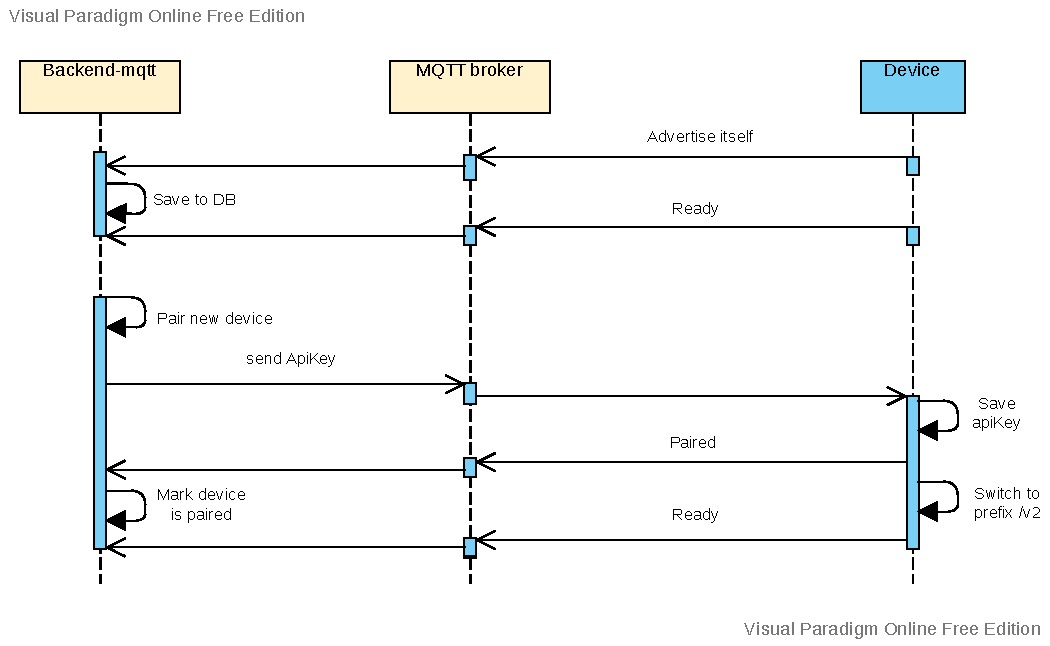
\includegraphics[width=\textwidth]{img/communication_part1.pdf}
    \caption{Diagram spárování zařízení}
\end{figure}
